\RequirePackage[]{optional}

\opt{slides}{
% Following for presentation mode
\documentclass[10pt]{beamer}
\usepackage{xmpmulti}
%usetheme{Berlin}
}
\opt{notslides}{
% Following for notes mode
\documentclass{article}
\usepackage{beamerarticle}
\usepackage{a4wide}
\usepackage{graphicx}
}

% Following for all modes
%\usepackage{auto-pst-pdf}
%\usepackage{pst-pdf}

\parindent=0ex
\parskip=1ex
\newcommand{\conv}{\ast}

\title{Fourier series and an RC circuit}
\author{}
\date{}

\begin{document}
%\mode<article>{\setbeamertemplate{frametitle}{}}  % no frametitles

\begin{frame}
\titlepage
\end{frame}

\mode<article>{{\bf \LARGE Fourier series and an RC circuit}}

\begin{frame}
  \frametitle{Circuit}
  Resistor $R$ in series with capacitor $C$, input $x(t)$ is
  voltage across combination, output $y(t)$ is voltage across
  capacitor.

  Resistor:
  \begin{equation*}
    v_r(t) = R i(t)
  \end{equation*}
  Capacitor:
  \begin{equation*}
    i(t) = C \frac{d}{dt} v_c(t)
  \end{equation*}
  and
  \begin{equation*}
    v(t) = v_c(t) + v_r(t)
  \end{equation*}
  Eliminating $i(t)$ and letting $v(t) = x(t)$ and $y(t) = v_c(t)$ gives
  DE
  \begin{equation*}
    x(t) = RC \frac{dy(t)}{dt} + y(t)
  \end{equation*}
\end{frame}

\begin{frame}
  \frametitle{System interpretation}
  The system is linear (linear constant coefficient DE), and
  therefore has an impulse response $h(t)$.  (Don't yet know how to find
  it.)

  The input/output relationship can therefore be written in the
  form
  \begin{equation*}
    y(t) = h(t) \conv x(t)
  \end{equation*}

  Input complex exponential $x(t) = c_1 e^{j \omega_0 t}$:
  \begin{align*}
    y(t) &= \int_{-\infty}^{\infty} h(\lambda) x(t-\lambda)
    d\lambda = \int_{-\infty}^{\infty} h(\lambda)
    c_1 e^{j \omega_0 (t-\lambda)} d\lambda \\
    &= \left( c_1 \int_{-\infty}^{\infty} h(\lambda)
    e^{-j \omega_0 \lambda} d\lambda \right) e^{j \omega_0 t}
    = d_1 e^{j \omega_0 t}
  \end{align*}
\end{frame}

\begin{frame}
  \frametitle{Finding output coefficients}
  Return to DE:
  \begin{equation*}
    x(t) = RC \frac{dy(t)}{dt} + y(t)
  \end{equation*}
  Consider input $x(t) = c_1 e^{j \omega_0 t}$.  Know the output
  is of the form $y(t) = d_1 e^{j \omega_0 t}$.  Coefficient $c_1$
  is known: want to find $d_1$.

  Substitute into DE and solve:
  \begin{gather*}
    c_1 e^{j \omega_0 t} = RC \frac{d}{dt} \left[ d_1 e^{j \omega_0 t}
    \right] + d_1 e^{j \omega_0 t} \\
    \Longrightarrow
    c_1 e^{j \omega_0 t} = j \omega_0 RC d_1 e^{j \omega_0 t}
    + d_1 e^{j \omega_0 t} \\
    \Longrightarrow
    c_1 = (j \omega_0 RC + 1) d_1
  \end{gather*}
  So
  \begin{equation*}
    d_1 = \frac{1}{1 + j \omega_0 RC} c_1
  \end{equation*}

\end{frame}

\begin{frame}
  \frametitle{Multiple component signal}
  Input complex exponential $x(t) = c_1 e^{j \omega_0 t}
  + c_2 e^{j 2 \omega_0 t}$:
  \begin{align*}
    y(t) &= \int_{-\infty}^{\infty} h(\lambda) x(t-\lambda)
    d\lambda \\
    &= \int_{-\infty}^{\infty} h(\lambda)
    c_1 e^{j \omega_0 (t-\lambda)} d\lambda +
    \int_{-\infty}^{\infty} h(\lambda)
    c_2 e^{j 2 \omega_0 (t-\lambda)} d\lambda \\
    &= \left( c_1 \int_{-\infty}^{\infty} h(\lambda)
    e^{-j \omega_0 \lambda} d\lambda \right) e^{j \omega_0 t} \\
    &\qquad \qquad \qquad \qquad +
    \left( c_2 \int_{-\infty}^{\infty} h(\lambda)
    e^{-j 2 \omega_0 \lambda} d\lambda \right) e^{j 2 \omega_0 t}
    \\
    &= d_1 e^{j \omega_0 t} + d_2 e^{j 2 \omega_0 t}
  \end{align*}
  Complex exponentials in, complex exponentials out at same
  frequencies.  Only need to find the coefficients $d_1$ and $d_2$
  given $c_1$ and $c_2$
\end{frame}

\begin{frame}
  \frametitle{Coefficients for multi-component signal}
  {\it You} can ({\it and should}) do same for two-component signal.  Let
  \begin{equation*}
    x(t)= c_1 e^{j \omega_0 t} + c_2 e^{j 2 \omega_0 t},
  \end{equation*}
  $y(t)$ must be of form
  \begin{equation*}
    y(t)= d_1 e^{j \omega_0 t} + d_2 e^{j 2 \omega_0 t},
  \end{equation*}
  substitute into the DE and solve (algebraically!) for $d_1$ and $d_2$.

  In general, if input and output are
  \begin{equation*}
    x(t) = \sum_{k=-\infty}^{\infty} c_k e^{j k \omega_0 t}
    \qquad \text{and} \qquad
    y(t) = \sum_{k=-\infty}^{\infty} d_k e^{j k \omega_0 t},
  \end{equation*}
  then
  \begin{equation*}
    d_k = \frac{1}{1 + j k \omega_0 RC} c_k
  \end{equation*}

\end{frame}

\begin{frame}
  \frametitle{In general}
  If there is a LCCDE linking inputs and outputs, the FS
  coefficients for input and output will be found to obey
  \begin{equation*}
    d_k = H(k \omega_0) c_k
  \end{equation*}
  where for the RC circuit we have
  \begin{equation*}
    H(\omega) = \frac{1}{1 + j \omega RC}
  \end{equation*}
  To work out how a signal is modified by the circuit, only need to
  know the values of $H(\omega)$ at the frequencies present

  $H(\omega)$ is just a complex number for each value of frequency
  $\omega$.  The plot of the magnitude and phase of $H$ as a
  function of $\omega$ is called the {\it Bode plot} of the
  system.
\end{frame}

\begin{frame}
  \frametitle{Bode plot for RC circuit}
  \begin{center}
    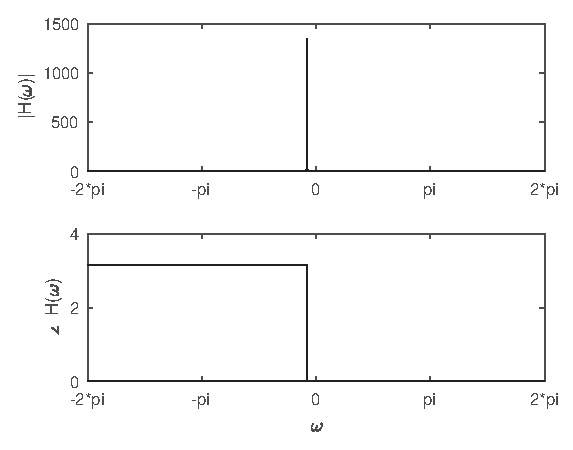
\includegraphics[width=9cm]{fs_rclpf_fig05}
  \end{center}
\end{frame}

\begin{frame}
  \frametitle{Observe}
  Time domain description of signals $x(t)$ and $y(t)$ $\longrightarrow$
  {\it differential equation} linking input and output of system.  Can solve
  for $y(t)$ given $x(t)$, but no intuition.

  Instead, think about signals as (weighted linear) combinations of complex
  exponentials (or combinations of frequencies)
  \begin{equation*}
    x(t) = \sum_{k=-\infty}^{\infty} c_k e^{j k \omega_0 t}
    \qquad \text{and} \qquad
    y(t) = \sum_{k=-\infty}^{\infty} d_k e^{j k \omega_0 t}
  \end{equation*}
  $\longrightarrow$ {\it algebraic equation} linking input and
  output:
  \begin{equation*}
    d_k = H(k \omega_0) c_k
  \end{equation*}
  Much easier to understand.
\end{frame}

\begin{frame}
  \frametitle{One component approximation to square wave}
  \begin{center}
    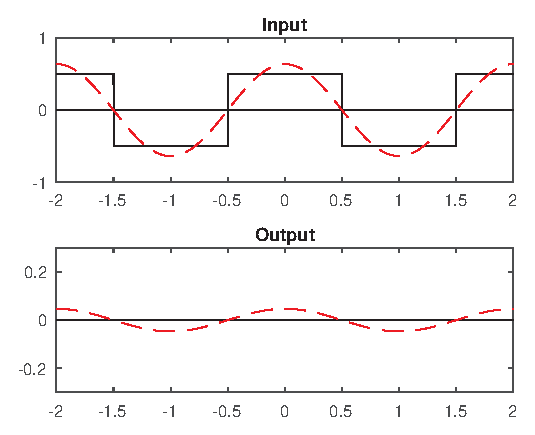
\includegraphics[width=9cm]{fs_rclpf_fig01}
  \end{center}
\end{frame}

\begin{frame}
  \frametitle{Two component approximation to square wave}
  \begin{center}
    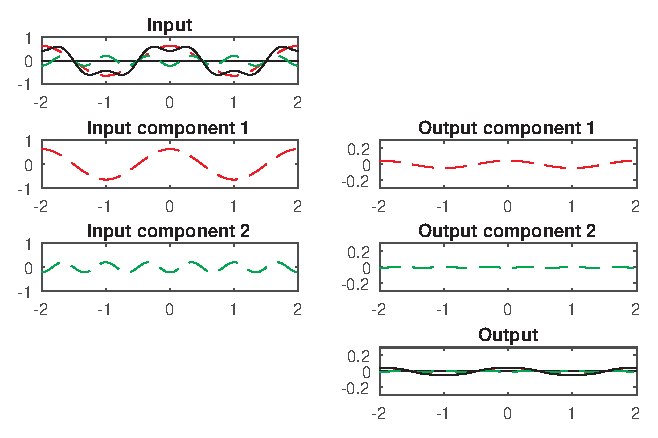
\includegraphics[width=9cm]{fs_rclpf_fig02}
  \end{center}
\end{frame}

\begin{frame}
  \frametitle{Many component approximation to square wave}
  \begin{center}
    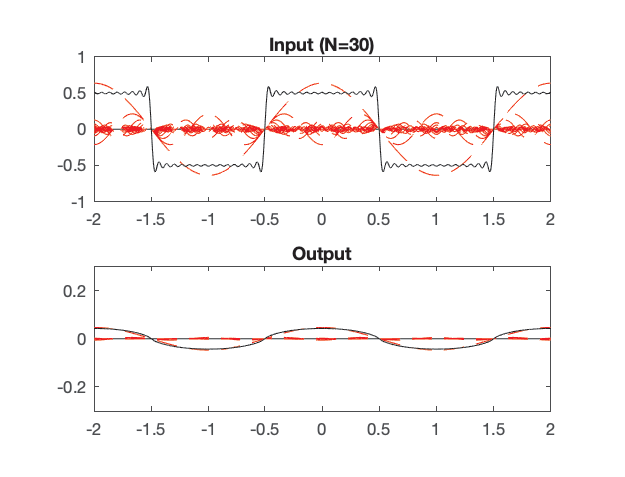
\includegraphics[width=9cm]{fs_rclpf_fig04}
  \end{center}
\end{frame}

\end{document}
